\documentclass[a4paper,11pt]{beamer}

\usepackage{préambule}

\begin{document}

\begin{frame}
	\begin{center}
		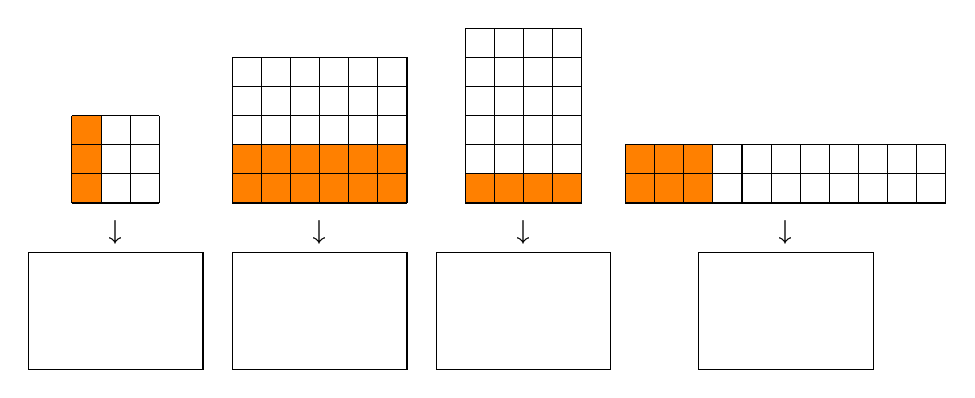
\begin{tikzpicture}[scale=0.37]
			\def\A{0};
			\def\B{7};
			\def\C{14};
			\def\D{23};

			\fill[orange] (\A+1.5,0) rectangle ++(1,3);
			\draw[xshift=0.5cm] (\A+1,0) grid ++(3,3);
			\node at (\A+3,-1) {↓};
			\draw (\A,-1.7) rectangle ++(6,-4);

			\fill[orange] (\B,0) rectangle ++(6,2);
			\draw (\B,0) grid ++(6,5);
			\node at (\B+3,-1) {↓};
			\draw (\B,-1.7) rectangle ++(6,-4);

			\fill[orange] (\C+1,0) rectangle ++(4,1);
			\draw (\C+1,0) grid ++(4,6);
			\node at (\C+3,-1) {↓};
			\draw (\C,-1.7) rectangle ++(6,-4);

			\fill[orange] (\D-2.5,0) rectangle ++(3,2);
			\draw[xshift=0.5cm] (\D-3,0) grid ++(11,2);
			\node at (\D+3,-1) {↓};
			\draw (\D,-1.7) rectangle ++(6,-4);
		\end{tikzpicture}
	\end{center}
\end{frame}


\end{document}